\documentclass[11pt]{article}

\usepackage[letterpaper,margin=1in]{geometry}

\usepackage{akteach}
\usepackage{amsmath}
\usepackage{amssymb}
\usepackage{enumerate}
\usepackage{keystroke}

\usepackage{natbib}
\newcommand{\doi}[1]{\href{http://dx.doi.org/#1}{doi: #1}}

\lstset{
  language=Bash,
  basicstyle=\ttfamily,
  commentstyle=\color{blue},
  stringstyle=\color{black},
}

\begin{document}

\akteachheader{High-Performance Scientific Computing (MATH-GA 2011/ CSCI-GA 2945)}%
{Homework Set 1}
\akteachsubheader{Due: September 12, 2012 $\cdot$ Out: September 5, 2012 }

\smallskip
Welcome to this semester's high-performance computing (``HPC'') class!
Remember that this class is about \emph{you} and how much you learn.
Please let us (the instructors) know what we can do to improve your
experience.

\smallskip This first assignment is meant to get you familiar with the
mechanics of this class, from asking questions, to running code on
NYU's HPC systems, to turning in homework. It'll also provide some
practice with C code. If you're unfamiliar with C or the tools we are
using, expect to spend a fair bit of time \emph{now} to catch up. This
will ensure that you won't be lost once we get to more complicated
things.

\smallskip
After the description of the assignment, you will find a few pages
that describe tools and procedures. Please make sure to read and
follow those carefully.

\bigskip
\akteachprobhead{Problem 1: Sorting with trees}

Write a program to sort a sequence of numbers using a
\weblink{https://en.wikipedia.org/wiki/Binary_tree}{binary tree}.
Define a \texttt{struct} to represent each node in
the tree.

\begin{enumerate}[a)]
\item Read a number \texttt{n} from the command line.
\item Allocate an array of size \texttt{n} integers. Using
  \weblink{https://www.gnu.org/software/libc/manual/html_node/ISO-Random.html}{\texttt{rand()}},
  fill it with \texttt{n} random integers. Make sure to use
  \texttt{srand()} to pick a seed, for reproducibility.
\item Build a binary tree from your array of numbers.
\item Output the sorted list to \texttt{stdout}, one integer
  per line.
\item Make sure you free all memory that you've allocated.
  (Yes, we will check!)
\item \label{part:tree-asymp}As an expression of \texttt{n}, what is the worst
possible runtime? What runtime do you expect typically?
What determines which case you fall into?
(Don't worry about constant factors or lower-order
terms in your expressions.)
\item \label{part:tree-runtime-discuss}Use this
\weblink{https://gist.github.com/3614336}{timing code}
to measure the run time you get for a range of list sizes.
Discuss how your observations match with your prediction
in part \ref{part:tree-asymp}).
\end{enumerate}

You will turn in your solution as a
`\weblink{https://en.wikipedia.org/wiki/Git_\%28software\%29}{\texttt{git}}'
repository (see below).
Your submission should be in a subdirectory `\texttt{problem-1}' and
should consist of at least these two files:

\begin{enumerate}
  \item Your program, as `\texttt{tree-sort.c}'.

    If your implementation consists of more than this
    one file, you must also supply a
    `\weblink{https://en.wikipedia.org/wiki/Make_\%28software\%29}{\texttt{Makefile}}'
    that will build your program when `\texttt{make}' is entered.

  \item A text file `\texttt{discussion.txt}' containing
    your solution to parts \ref{part:tree-asymp})
    and \ref{part:tree-runtime-discuss}) as plain
    text. (i.e. not Word, PDF, or some such)

    Your answer to each subproblem should be about a short paragraph.
\end{itemize}

\akteachprobhead{Problem 2: Matrix multiplication}

\begin{figure}

\end{figure}



Before you begin, please flip through the lecture slides again and
read the provided links for the things that seem even slightly
unfamiliar to you. All the blue-underlined phrases in the slides PDF
are clickable links. Likewise, we've provided many links in this
document to help you read up on things you might not already know.
\smallskip

For this first assignment, you will optimize a routine to multiply
square matrices. Matrix multiplication is a basic building block in
many scientific codes; and since it is an $O(n^3)$ algorithm, these
codes often spend a lot of their time in matrix multiplication.

\subsection*{Implementation}

The most naive code to multiply matrices is short, sweet, and slow:

\begin{lstlisting}
  for i = 1 to n
    for j = 1 to n
      for k = 1 to n
        C[i,j] = C[i,j] + A[i,k] * B[k,j]
      end
    end
  end
\end{lstlisting}

You need to write a \texttt{dgemm.c} that contains a function with the
following argument types in C:

\begin{lstlisting}[language=C]
void
square_dgemm(const unsigned M,
             const double *A, const double *B, double *C)
\end{lstlisting}

\begin{figure}

\begin{center}
  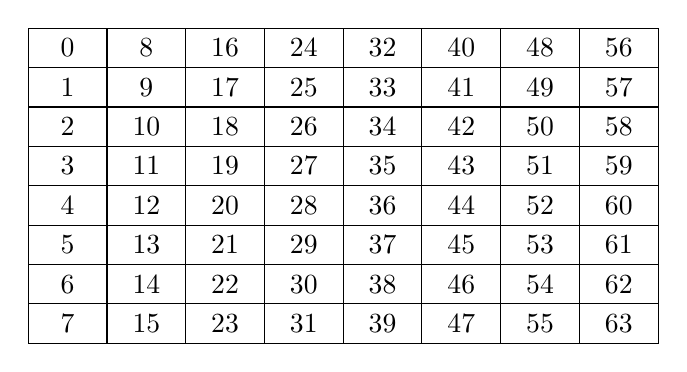
\begin{tikzpicture}[yscale=-0.5]
    \foreach \i in {0,1,...,7}
      \foreach \j in {0,1,...,7}
      {
        \draw (\i,\j) rectangle +(1,1) node [pos=0.5] {
          \pgfmathtruncatemacro{\res}{\i*8+\j}\res
        };
      }
  \end{tikzpicture}
\end{center}

\caption{Column-major matrix layout. The numbers in the cells
represent linear array indices.}
\label{fig:column-major}
\end{figure}

Note that the matrices are stored in
\weblink{http://en.wikipedia.org/wiki/Row-major_order}{column-major
order}, as shown in Figure \ref{fig:column-major}.  Also, your
program will actually be doing a multiply and add operation:

\[
  C \leftarrow C + A*B
\]

This homework set comes with a starter kit. (We will explain how you
can get it in the instructions later on.) You may look at the code in
\verb|basic_dgemm.c| in the kit if you are confused by what you need
to implement.

To tackle this assignment, you will need to understand the pattern in
which matrix multiplication references data. Start by understanding
the temporal access sequence of the naive version
\verb|basic_dgemm.c|, then understand the (also provided) blocked
version \verb|blocked_dgemm.c|.

Then, attempt to improve on performance by rearranging/splitting the
loops in the blocked implementation.  (This is called
``\weblink{http://en.wikipedia.org/wiki/Loop_tiling}{loop tiling}''.)
In addition, you might want to use a special treatment for the fringe
blocks that don't fully fill a block. Use the provided timing facility
in \texttt{timing.h} and \texttt{timing.c} to find out where time is
spent, and guide your efforts accordingly. (That is--if some part of
the algorithm is using 0.1 per cent of the running time, and you
manage to make it ten times faster, you have won nearly nothing.
Needless to say, you should avoid this.)

If you're ambitious or lost, the papers by
\citet{lam1991cache,bilmes1997optimizing,whaley_automated_2001} might
be of help.

\subsection*{Starting Out}

In the starter kit, we provide
\begin{itemize}
  \item an implementation of the trivial unoptimized matrix multiply
  code in C.

  You can find this implementation in \verb|basic_dgemm.c|.

  If you don't know C yet, try reading Sections 1 through 7 and 10
  of this
  \weblink{http://www.physics.drexel.edu/courses/Comp_Phys/General/C_basics/c_tutorial.html}{tutorial}.

  \item a basic blocked matrix multiply from which
  you can start your implementation.

  See \verb|blocked_dgemm.c| in the starter kit.

  \item a way to compare your routines to code optimized by
  ``professionals''--in this case, to the Intel Math Kernel Library
  (``\weblink{http://en.wikipedia.org/wiki/Math_Kernel_Library}{MKL}''),
  which provides an implementation of the
  \weblink{http://en.wikipedia.org/wiki/Basic_Linear_Algebra_Subprograms}{BLAS}
  (Basic Linear Algebra Subroutines) library. The BLAS is a standard
  interface for building blocks like matrix multiplication, and many
  computer vendors provide optimized versions of the BLAS.

  See \verb|blas_dgemm.c| in the starter kit.

  \item a ``Makefile'' that helps you build and run the sample
    code as well as your own code.
    \weblink{http://en.wikipedia.org/wiki/Make_(software)}{Make} is
    a program that aids in compiling software. It relies on a file
    called \texttt{Makefile}, which defines a number of
    \emph{targets}. These targets can then be built by typing
    \begin{lstlisting}
$ make <target>
\end{lstlisting}
    where you substitute the target name for \verb|<target>|.  Our
    makefile provides a number of targets--you can find their names by
    taking a look at the file. The Wikipedia page on make (as linked
    above) has more information, and the complete truth is in the
    \weblink{http://www.gnu.org/software/make/manual/html_node/index.html}{GNU
    make manual}.

\end{itemize}


We will be testing on and optimizing for the 2.33 GHz Intel Xeon E5345
processors on the NYU cluster ``Union Square'' (again, more info on
this machine and how to access it can be found below). These chips are
essentially the same as the Intel Q6600 mentioned a few times in
class, and like it, they are also quad-core processors (but you will
be using only one core for this assignment).

Once you have obtained your starter kit (as described below in the
section on \texttt{git}), you may follow the following session
transcript to actually run your code. Note that blue text after a hash
sign (``\texttt{\#}'') is a comment that does not need to be typed.
Command output is also visible. You can find the commands that were
typed by looking for these prompts:
\begin{lstlisting}
[ak177@login-0-0 hw1]$ ... command ...
\end{lstlisting}

And here is the transcript:

\begin{lstlisting}
# We're submitting an interactive job (-I) to a queue named `interactive' (-q).
[ak177@login-0-0 hw1]$ qsub -q interactive -I
qsub: waiting for job 2274407.hpc0.local to start
qsub: job 2274407.hpc0.local ready

10.0.1.240@o2ib:10.0.1.239@o2ib:/scratch on /scratch type lustre (rw,noauto,_netdev)
mgs-0-0-ib@o2ib2:/scratchy on /scratch.tmp type lustre (rw,noauto,_netdev)

# The job has started, and we're now logged into a compute node.
#
# We start out in the home directory, and thus need to change to the
# directory where the hw1 files are kept.
[ak177@compute-0-97 ~]$ cd where/ever/hw1/

# Next, we compile the code. `matmul-blas' is the BLAS version of
# the code. `matmul' and `matmul-blocked' also exist.
#
# We compile the code using `make'.
[ak177@compute-0-97 hw1]$ make matmul-blas
cc -c  "-DCOMPILER=\"cc\"" "-DFLAGS=\"-O2\"" matmul.c
cc -c  "-DCOMPILER=\"cc\"" "-DFLAGS=\"-O2\"" timing.c
cc -c  "-DCOMPILER=\"cc\"" "-DFLAGS=\"-O2\"" blas_dgemm.c \
  -I/share/apps/intel/Compiler/11.1/046/mkl//include
cc -o matmul-blas matmul.o timing.o blas_dgemm.o  -lm -lrt
  -L/share/apps/intel/Compiler/11.1/046/mkl//lib/em64t/
  /share/apps/intel/Compiler/11.1/046/mkl/lib/em64t/libmkl_solver_ilp64_sequential.a
  -Wl,--start-group -lmkl_intel_ilp64 -lmkl_sequential
  -lmkl_core -Wl,--end-group -lpthread

# The Makefile did some complicated things involving the C compiler (`cc').
# There were no error messages, so it looks like everything worked.
#
# Now let's try and run the resulting binary.
[ak177@compute-0-97 hw1]$ ./matmul-blas
./matmul-blas: error while loading shared libraries:
  libmkl_intel_ilp64.so: cannot open shared object file: No such file or directory

# That did not work out--the machine cannot find the MKL library, so
# we need to make it available.
[ak177@compute-0-97 hw1]$ module load mkl/11.1.046

# We retry the run.
[ak177@compute-0-97 hw1]$ ./matmul-blas
Compiler:       cc
Options:        -O2
Description:    System BLAS dgemm.

Size: 31        mflop/s: 4438.78
#... more lines like this ...
Size: 769       mflop/s: 8312.88

# Perfect. Now let's save the output to a file called `timing.raw'.
[ak177@compute-0-97 hw1]$ ./matmul-blas > timing.raw
# nothing appears to happen for a minute or two

# Next, this is how we can generate a plot from the data in
# `timing.raw'.
[ak177@compute-0-97 hw1]$ make timing.ps
awk '/Size/ { print $2 " " $4 }' timing.raw > timing
echo "set term postscript; set output 'timing.ps';" \
    | gnuplot - timing.gnuplot
gnuplot> Terminal type set to 'postscript'
Options are 'landscape noenhanced monochrome blacktext \
   dashed dashlength 1.0 linewidth 1.0 defaultplex \
   palfuncparam 2000,0.003 \
   butt "Helvetica" 1
[ak177@compute-0-97 hw1]$
\end{lstlisting}
By this time, a file \texttt{timing.ps} has been created that shows a
plot of your performance data.

If you would like more automation (and know roughly what a shell
script is), you may investigate the \texttt{run-*} makefile targets.

\subsection*{Submission}

In your submission, we expect to find:

\begin{itemize}
  \item a file named \texttt{writeup.pdf}, which describes your work.

  In particular, please include
  \begin{itemize}
    \item your name,
    \item the optimizations used or attempted,
    \item the results of those optimizations, and
    \item your explanation for any odd behavior (e.g., dips) in performance.
  \end{itemize}

  You should compare all versions of your code, including intermediate
  ones, to
  \begin{itemize}
    \item the supplied \verb|basic_dgemm.c| and
    \item the initial, supplied \verb|blocked_dgemm.c| and
    \item the (also supplied) BLAS DGEMM from the
      Intel Math Kernel libraries.
  \end{itemize}

  All your comparisons should include a plot showing MFlop/s along the
  $y$-axis and the size of the matrix along the $x$-axis. Since the
  exact number of floating point operations carried out is often hard
  to count exactly, we will just use $2n^3$ as a reasonable estimate.

  As much as possible, you should include explanations of the features
  (dips, ramps, etc.) seen in these graphs. Your explanations should
  rely on your knowledge of processor architecture and the memory
  hierarchy.

  Also note that graphs with different $x$ axes (tile size, etc.)
  might help you understand and explain some aspects of the
  performance you observe.

  \item your final \verb|dgemm.c|, buildable and runnable through the
  provided \texttt{Makefile} system.
\end{itemize}


\bibliographystyle{abbrvnat}
\bibliography{hw1}

\clearpage

\akteachheader{Machine Access and Homework Submission}{Helpful Hints}

% -----------------------------------------------------------------------------
\subsection*{Getting Help}

If you are having technical trouble, if some instructions here fail to
work for you, or if things just seem confusing, don't despair: There's
plenty of help available.

First of all, please make sure you are subscribed to the class mailing
list. Someone might have had the same problem as you (and ideally
already solved it).  If you are subscribing an address ending in
\texttt{nyu.edu}, you may do so yourself at
\weblink{http://lists.tiker.net/listinfo/hpc12}{the
list's web page}. If you'd like to subscribe a non-NYU address, email
Andreas to subscribe you. The list has
\weblink{http://lists.tiker.net/private/hpc12/}{archives}
where you can check if you've missed anything important.

If your problem concerns the NYU HPC machines, try checking the
\weblink{https://wikis.nyu.edu/display/NYUHPC}{NYU HPC Wiki}.
If that (and perhaps a bit of Googling around) doesn't answer your
question, send email to
\begin{quote}
  \href{mailto:hpc12@tiker.net}{\texttt{hpc12@tiker.net}}.
\end{quote}

If you would like to discuss a technical issue (i.e. one that isn't
directly related to you), please do not email us (the instructors).
Instead, please send a message to the mailing list, where we (and your
peers) will be more than happy to assist.  Thanks!

Again, welcome, and we hope you'll have an enjoyable and worthwhile
experience in this class.

\begin{note}
All homework in this class will be UNIX-based. While you
may be able to get by with Windows on your personal machine, for
familiarity and ease of use we \emph{strongly} recommend also using
Linux/Unix/OS~X on your own computer.
To make this easier, we've provided a virtual machine that lets you
play with all the technologies we'll touch on in this class. (C,
OpenMP, MPI, OpenCL) This allows you to get started immediately.
You'll need to install \weblink{http://virtualbox.org}{Virtualbox}
and then grab the machine image from

\begin{quote}
  \url{http://bit.ly/hpc12-vm}
\end{quote}

are providing a virtual machine image that
contains all the tools you'll need for this class.
\end{note}

% -----------------------------------------------------------------------------
\subsection*{Logging into Union Square (\texttt{usq})}

All access to the high-performance machines at NYU goes through
\texttt{hpc.nyu.edu} (a.k.a. the ``bastion host''). You may log in using
\weblink{http://en.wikipedia.org/wiki/Secure_Shell}{SSH}:
\begin{lstlisting}
your-machine$ ssh NETID@hpc.nyu.edu
\end{lstlisting}
Your user name on this machine is your NYU NetID (the same one you use
to log into NYUHome). Likewise, your password is the same one you use
to access NYUHome.

\begin{note}
In this document, the dollar sign ``\texttt{\$}'' represents a
command prompt. The actual command you need to type follows after that. For
clarity, a symbolic host name may precede the dollar sign.
\end{note}

Most Linux distributions and OS~X should come with \texttt{ssh}
pre-installed.  If you are using a Windows machine, you may use
\weblink{http://www.chiark.greenend.org.uk/~sgtatham/putty/}{PuTTY}.

The first time you log in, the system will warn you that it does not
know about \texttt{hpc.nyu.edu}; just say ``yes'' to log in anyhow and
permanently accept this machine as a known host.

From the bastion host, the only thing you can do is use SSH to access other
machines. To reach Union Square, type
\begin{lstlisting}
hpc$ ssh usq
\end{lstlisting}
The first time you log in, you will again get a warning from
\texttt{ssh}. Proceed as above.

After you give your password, you will be logged into \texttt{usq}.
The first time you log in, you will be prompted to set up an SSH key
pair.  This key pair serves two purposes: First, it will
allow your jobs to access the cluster's compute nodes on which they
are supposed to run. Second, it will act as your key to the class
collaboration space (see below).

Just hit \Enter when prompted for a passphrase. The interaction will
look something like this:

\begin{lstlisting}
It doesn't appear that you have set up your ssh key.
This process will make the files:
     /home/NETID/.ssh/id_rsa.pub
     /home/NETID/.ssh/id_rsa

Generating public/private rsa key pair.
Enter file in which to save the key (/home/NETID/.ssh/id_rsa):
Enter passphrase (empty for no passphrase):
Enter same passphrase again:
Your identification has been saved in /home/NETID/.ssh/id_rsa.
Your public key has been saved in /home/NETID/.ssh/id_rsa.pub.
The key fingerprint is: ...
\end{lstlisting}

Now you are logged into the cluster!

If you are unsure of what to type next, consider taking a look at
\weblink{http://people.ischool.berkeley.edu/~kevin/unix-tutorial/toc.html}{a
friendly Unix tutorial} (recommended). (Googling for ``unix tutorial''
gives plenty more options.) Note that the tutorial recommends the
``\texttt{pico}'' editor, which is unavailable at NYU. You may instead
use ``\texttt{nano}'', which works identically aside from its
different name.

Also, note that you will get a
\weblink{http://en.wikipedia.org/wiki/Bash_(Unix_shell)}{bash} shell
by default. If you are used to the C shell, ask us on how to change
that. Note that the class homework starter kit contains scripts that
assume you are using the default \texttt{bash}. You might have to
change those if you do switch to the C shell.  (If this was
mumbo-jumbo to you, forget about it.)

At some later point, we will also use what NYU calls the ``CUDA
cluster'', \texttt{cuda.es.its.nyu.edu}. Most procedures for that
machine are the same as for \texttt{usq}, but you will have to
say \texttt{cuda} whenever the instructions call for \texttt{usq}.

% -----------------------------------------------------------------------------
\subsection*{Moving files to and from NYU HPC}

See this
\weblink{https://wikis.nyu.edu/display/NYUHPC/Managing+Data\#ManagingData-Movingfilesto\%2Ffromthecluster}{wiki page} on how to move data back and forth between your computer and the
HPC clusters.

Note that if you have access to a machine that has SCP/SFTP accessible
from the outside network (such as \texttt{access.cims.nyu.edu}), you
can avoid the tedious two-step process via the bastion host by
initiating file transfers \emph{from} the clusters.

Here's an example of this usage to copy files \emph{from the cluster}
to somewhere else:
\begin{lstlisting}
cluster$ scp  -rp  <file or pattern>  <outside-user>@<outside-host>:<dest. path rel. to home>
Password:...
<Progress>
cluster$
\end{lstlisting}
(Spaces shown for clarity.) Please make sure to not forget the colon
after the outside host!  And this is how you copy outside files onto
the cluster:
\begin{lstlisting}
cluster$ scp  -rp  <outside-user>@<outside-host>:<source path rel. to home>  .
Password:...
<Progress>
cluster$
\end{lstlisting}
Again, please mind the dot and the colon.

% -----------------------------------------------------------------------------
\subsection*{Compiling and Running Serial Code}

Please see the corresponding
\weblink{https://wikis.nyu.edu/pages/viewpage.action?pageId=4587655}{HPC
wiki page}, which should have most of the information you need.

As you saw in the session transcript above, we will generally be using
the HPC system's \texttt{interactive} queue. This queue is for short,
low-processor count jobs. Once we tackle more ambitious assignments,
we will likely need to also use different queues. Once we get to that
point, this will be brought up in class.

% -----------------------------------------------------------------------------
\subsection*{Using \texttt{git} for Homework and Collaboration}

We expect you to use the
\weblink{http://en.wikipedia.org/wiki/Distributed_revision_control}{distributed
version control} system \weblink{http://git-scm.org}{git} for
developing and turning in solutions to your homework. Like compilers,
debuggers, and build tools, version control systems are central to
most present-day software development. By having you use \texttt{git},
we hope to be able to give you some familiarity with such tools.

Along with the tool itself, we will use a central collaboration space,
\url{http://forge.tiker.net}, which works like the big, public
development hubs SourceForge, Google Code, or Github. You will set up
an account there and create a new ``project'' for every assignment
(and your final project). The collaboration space provides the
following functions in our class:
\begin{itemize}
  \item We will grade what is on \texttt{forge} after the homework
  deadline. As a result, you definitely want to upload your finished
  assignment.
  \item It will allow you to collaborate on your final project with a friend.
  \item If you are having an issue with your current code, you may
  upload it and ask the instructors to view it on \texttt{forge}.
  \item It provides an easy conduit to get code from the HPC clusters
  onto another machine and back.
\end{itemize}

\begin{note}
Your account on \texttt{forge} is initially limited to
about 50 megabytes, with more available if needed. Please do not check
in large data files before discussing your needs with Andreas.

Your accounts on \texttt{forge} and the data you store there will be
removed on February 1, 2011. Please back up your code and data before
this date.
\end{note}

To use
\texttt{git} on the NYU machines, you need to type
\begin{lstlisting}
module load git/gnu/1.7.2.3
\end{lstlisting}
To avoid having to type this every time, consider adding this command
to the \texttt{.bashrc} (note the dot!) file in your home directory.

NYU uses the software ``\weblink{http://modules.sourceforge.net/}{Environment
Modules}'' to manage a variety of software installed on its clusters.
By typing the `\texttt{module load}' command above, you have already
used this system to allow you to use \texttt{git}. You may type
\begin{lstlisting}
module avail
\end{lstlisting}
to find which other software modules are available. In particular, you
may choose to use the
\weblink{http://en.wikipedia.org/wiki/Intel\_C\%2B\%2B\_Compiler}{Intel
Compilers} instead of the default GNU ones. Like \texttt{git}, these
compilers are activated through the \texttt{module load} commands. The
NYU HPC Wiki describes these compilers in more detail.

Next, inform \texttt{git} of your name and email address:
\begin{lstlisting}
$ git config --global user.name "Your Name Comes Here"
$ git config --global user.email you@yourdomain.example.com
\end{lstlisting}

To access the class-wide collaboration space, go to
\url{http://forge.tiker.net}. Click ``Sign in or create account''.
Please use your NetID as your user name. The system will confirm your
email address by sending you a confirmation key.

\begin{note}
We have found that these confirmation emails often get flagged as spam
by a variety of spam filters. Please check your spam folder if the
email doesn't seem to have arrived within a few minutes.
\end{note}

Once you complete this
verification step, fill out your name, password, and click ``Enable my
Account''. Please do \emph{not} use a valuable password here, in
particular \emph{not} your NYU-wide one. You are now logged into
\texttt{forge.tiker.net}.

Next, while you are logged into \texttt{usq}, type
\begin{lstlisting}
usq$ cat $HOME/.ssh/id_rsa.pub
\end{lstlisting}
This will print a few lines (technically, just one wrapped line) that
looks like this:
\begin{lstlisting}
ssh-rsa AAAABw...vM3XdIbZWwmXH/iNbFWEhZw== NETID@login-0-1.local
\end{lstlisting}
Once you are logged into \texttt{forge}, click your name in the top
left corner. Click ``Update your account'' on the left and then paste
the line returned above into the field that says ``Add public key''.
Click ``Update your Account''. The key update may take up to two
minutes to fully complete, so if any steps involving git below fail,
wait for two minutes, and then try again.
This completes the setup steps that are only required once.

Next, you may clone the starter repository for homework 1:
\begin{lstlisting}
git clone ssh://git@forge.tiker.net:2234/hw1.git
\end{lstlisting}
You now have a completely independent copy of this repository, and you
may change any and all files in there and commit your code as you go
along. (Note that these commits will \emph{not} automatically end up
on the server--see below!) Pleas take a look at the
\weblink{http://www.kernel.org/pub/software/scm/git/docs/gittutorial.html}{git
tutorial}. You should at least be familiar with the usage of the commands
\begin{itemize}
  \item \texttt{git status}
  \item \texttt{git add}
  \item \texttt{git commit}
  \item \texttt{git log}
  \item \texttt{git diff}
\end{itemize}
Note that you do not need to use \texttt{git init} as you will always
work on an exisiting repository that you copied (``cloned'') from
somewhere else.  One piece of advice: Commit frequently--at least once
for every milestone you complete along the way. This allows you
to go back to a working version if you've made changes that you would
like to get rid of.

The next steps will create a possibility for you to upload changes
back to \texttt{forge}.  To do this, navigate to
\url{http://forge.tiker.net/} (or click on ``Project List'' if you're
already there) and, once there, click on ``Create Project''. You may
choose a name for the new repository, as well as a ``shortname'' (i.e.
Unix-level name). If you are turning in your first homework set,
please choose this shortname as ``\texttt{hw1-netid123}''.  For the
``Project Creation Key'', enter ``\texttt{nyuhpc10}'' and make sure
the ``Private repository'' box is checked. If necessary, you may also
add co-owners and collaborators by their NetID. Once you click
``Create Project'', your repository is ready to go.

To upload the (committed) state of your git repository to
\texttt{forge}, change to the repository directory and type
\begin{lstlisting}
$ git remote add forge ssh://git@forge.tiker.net:2234/<shortname>.git
$ git push forge master
\end{lstlisting}
If everything worked out, you should get output like this:
\begin{lstlisting}
Counting objects: 34, done.
Delta compression using up to 8 threads.
Compressing objects: 100% (21/21), done.
Writing objects: 100% (34/34), 8.25 KiB, done.
Total 34 (delta 12), reused 30 (delta 11)
To ssh://git@forge.tiker.net:2234/hw1-ak177.git
 * [new branch]      master -> master
\end{lstlisting}
The first command sets up a symbolic name \texttt{forge} for the
repository address, and the second one actually performs the upload.
Next time you want to upload your code, you may therefore simply say
\begin{lstlisting}
$ git push forge master
\end{lstlisting}
You may also navigate to \url{http://forge.tiker.net}, pick your
project from the list, navigate to the ``Source'' tab and verify that
the right version of the code is checked in.

\end{document}
